% Created 2017-10-05 Thu 16:11
% Intended LaTeX compiler: pdflatex
\documentclass[journal=ancac3,manuscript=article,email=true,hyperref=true,keywords=true]{achemso}

%manuscript=suppinfo

% \usepackage{minted}
% \usepackage{graphicx}
%\usepackage{float}
%\usepackage{xcolor}
%\usepackage{amsmath}
%\usepackage{amssymb}
%\usepackage{fontspec}
%\renewcommand{\figurename}{}

\setkeys{acs}{usetitle = true}
\usepackage{lmodern}
\usepackage{amsmath}
\usepackage{graphicx}
\usepackage{hyperref}
\usepackage{caption}
\usepackage[T1]{fontenc}
\usepackage{longtable}
\usepackage{footnote}
\renewcommand{\sfdefault}{cmr}

%\renewcommand{\thefigure}{Supplementary Figure \arabic{figure}}
\usepackage{float}

\renewcommand{\figurename}{\bf Supplementary Figure}
\renewcommand{\tablename}{\bf Supplementary Table}
%\renewcommand{\bibname}{Supplementary References}

\author{Dale Hughes}
\affiliation{School of Mathematics and Physics, Queen's University Belfast, BT7 1NN, United Kingdom}
\altaffiliation{D. H. and T. T. Contributed equally to this work}

\author{Tian Tian}
\affiliation{Institute for Chemical and Bioengineering, ETH Z{\"{u}}rich, Vladimir Prelog Weg 1, CH-8093 Z{\"{u}}rich, Switzerland}
\altaffiliation{D. H. and T. T. Contributed equally to this work}

\author{Declan Scullion}
\affiliation{School of Mathematics and Physics, Queen's University Belfast, BT7 1NN, United Kingdom}

\author{Lu Hua Li}
\affiliation{Institute for Frontier Materials, Deakin University, Waurn Ponds, Victoria, Australia}

\author{Chih-Jen Shih}
\affiliation{Institute for Chemical and Bioengineering, ETH Z{\"{u}}rich,  Vladimir Prelog Weg 1, CH-8093 Z{\"{u}}rich, Switzerland}

\author{Jonathan N. Coleman}
\affiliation{School of Physics, Centre for Research on Adaptive Nanostructures and Nanodevices (CRANN) and Advanced Materials and BioEngineering Research (AMBER), Trinity College Dublin, Dublin 2, Ireland.}

\author{Manish Chhowalla}
\affiliation{Materials Science and Engineering, Rutgers University, 607 Taylor Road, Piscataway, New Jersey 08854, USA.}

\author{Elton J. G. Santos}
\email{e.santos@qub.ac.uk}
\affiliation{School of Mathematics and Physics, Queen's University Belfast, BT7 1NN, United Kingdom}
\keywords{two-dimensional materials, dielectric constant, first-principles calculation, band gap, binding energy}
\date{}

\title{Supplementary Information: \\
Universal Understanding of the Dielectric Constants of Two-Dimensional Materials}
\begin{document}

%\newpage{}

\pagebreak{}

\section{Table of Contents}

1. Supplementary Note 1: 2D-Moss relations at different levels of theory: PBE, $G_{\rm 0}W_{\rm 0}$ \\ 
%
2. Supplementary Figure 1: Simulations using PBE functional. \\
%
3. Supplementary Figure 2: Simulations using many-body $G_{\rm 0}W_{\rm 0}$ approach \\ 
%
4. Supplementary Figure 3: Model predictions at PBE level  \\ 
% 
5. Supplementary Figure 4: Hybrid functional versus many-body band gaps  \\ 
%
6. Supplementary Note 2: Additional discussions on Moss' description of photoconductivity \\
%
7. Supplementary Figure 5: Normalization of band gaps using $E_g/\varepsilon_{\parallel}^2$ \\ 
%
8. Supplementary Note 3: Linking excitonic binding energies and dielectric constants  \\
%
9. Supplementary Figure 6: Scaling relations between dielectric constants and excitonic binding energies \\ 
%
%Include here the part from main text. 
10. Supplementary Figure 7: A second model to extract dielectric constants \\
%
11. Supplementary Note 4: Multiscale calculations between monolayer and bulk \\ 
%
12. Supplementary Figure 8: Relationship between the 2D and 3D dielectric constants \\ 
%
%13. Supplementary Note 5: Derivation of  $\varepsilon^{\mathrm{2D}} =   \displaystyle 1 + \frac{1}{4 \pi \varepsilon_{0}}
 %                     \frac{4 e^2 \pi \hbar^2}{m_e^2 E_g^2} J_{cv} P_{cv}^{2}$ \\
%
13. Supplementary Figure 9: Quantum capacitance over valence states \\
%
14. Supplementary Table 1: Comparison between dielectric constants of 2D materials and 3D materials \\ 
%
15. Supplementary Table 2: Fitting parameters for $C_{Q}$ \\ 
%
16. Supplementary Table 3: Database of \textit{Ab initio} calculations using HSE06 hybrid functional \\
%
17. Supplementary Figures 10-61: DOS-calculation results using HSE06 functional plus self-consistent spin-orbit coupling \\
%
18. Supplementary References \\

%4. Figure S4: Comparison between $\varepsilon_{\parallel}$ from HSE06 method and estimated from $E_{\mathrm{g}}$ \\


\pagebreak{}

%\subsubsection{Supplementary Figure 1: Summary of systems studied and group separation}

%{\bf Figure S1: Summary of systems studied and group separation}

%\begin{figure}[H]
%\centering
%\includegraphics[width=0.80\linewidth]{fig1_v122017_ink.pdf}
%\caption{\label{fig-S1} 
%{\bf 2D geometries and periodic table. a}, Schematic of the geometries of the 2D materials included in our database. 
%Compounds include monochalcogenides, dichalcogenides at the most common phases, such as  
%2H (P\(\bar{6}\)m2 space group) and 1T (P3m1 space group); 
%graphene derivatives (graphane, f-graphene); phosphorene, h-BN, 
%halides (CdX$_2$) and popular organic-inorganic perovskites (CH$_3$NH$_3$PbBr$_3$). 
%{\bf b}, Periodic table showing the main elements utilized in our high-throughput screening, and the classification of the groups accordingly to their scaling relationships. Several materials have resulted 
%to be metals (group 5, 7, 8, 9, 11) with dichalcogenide formula, which were not included here.  
%}
%\end{figure}
%
%
%\pagebreak{}


\subsubsection{Supplementary Note 1: 2D-Moss relations at different levels of theory: PBE, $G_{\rm 0}W_{\rm 0}$}

%Figure S2: PBE results for \(\varepsilon_{\parallel}\) and \(\varepsilon_{\perp}\) versus band gaps}

To demonstrate the validity of the Moss relation for 2D materials we have performed calculations 
at different levels of theory, such as using plain PBE functional (Supplementary Figure \ref{fig-S2}), HSE06 hybrid functional (Figure 1) and many-body $G_{\rm 0}W_{\rm 0}$ (Supplementary Figure \ref{fig-S3}). Despite of the method utilized all three approaches resulted in clear dependence of $\varepsilon_{\parallel}$ as a 
function of band gaps, and no-dependence of $\varepsilon_{\perp}$. Slight variations of the fitting parameters are observed, which are expected due to the different levels of treatment of the electronic and dielectric properties of the layers. It is worth mentioning however that better accuracy between calculated magnitudes of $\varepsilon_{\parallel}$ and $\varepsilon_{\perp}$ 
are obtained at HSE06 and $G_{\rm 0}W_{\rm 0}$. 

%It should be noted that simulations carried out at the level of PBE functional resulted in considerably larger differences between the model predictions and calculated \(\varepsilon_{\parallel}\) and \(\varepsilon_{\perp}\) (see Supplementary Figure \ref{fig-S4}). Deviations from either a purely linear fitting without a finite cumulative factor at the model, or magnitudes that differ by more than $\sim$24\% between simulations and scaling relations are observed. 
 

\begin{figure}[H]
\centering
\includegraphics[width=1.05\linewidth]{figure1S_v010318ink.pdf}
\caption{\label{fig-S2}
{\bf Simulations using PBE functional. a-b}, PBE results for the in-plane $\varepsilon_{\parallel}$ and out-of-plane $\varepsilon_{\perp}$  
dielectric constants, respectively, for monolayer materials as a function of the electronic band gap. 
Similar classification of the 2D materials as in {\bf Figure 1}  
is used for comparison: linear (green circles) and power (orange squares) groups. 
Orange and green lines are fits 
to $\varepsilon_{\parallel}=3.36/E_{g}^{0.71}$ and 
$\varepsilon_{\parallel}=7.79-2.15E_{g}$, respectively, in {\bf a}. 
The original 3D-Moss relation, $\varepsilon_{\parallel}=9.74/E_{g}^{0.50}$, 
between the dielectric constant of bulk semiconductors and band gap 
is shown as faint blue line.  
Dataset for $\varepsilon_{\perp}$ in {\bf b} are fitted using straight lines, 
$\varepsilon_{\perp}=1.21+(0.05)E_{g}$ (green) and $\varepsilon_{\perp}=1.60-(0.12)E_{g}$ (orange). 
The inset in {\bf b} shows the spatial definition of both $\varepsilon_{\perp}$ and $\varepsilon_{\parallel}$. 
}
\end{figure}

\begin{figure}[H]
\centering
\includegraphics[width=1.05\linewidth]{figureS_GW_gap_moss_v021218ink.pdf}
\caption{\label{fig-S3}
{\bf Simulations using many-body $G_{\rm 0}W_{\rm 0}$ approach. a-b}, $G_{\rm 0}W_{\rm 0}$ results for the in-plane $\varepsilon_{\parallel}$ and out-of-plane $\varepsilon_{\perp}$  
dielectric constants, respectively, for monolayer materials as a function of the electronic band gap. 
Similar classification of the 2D materials as in {\bf Figure 1}
is used for comparison: linear (green circles) and power (orange squares) groups. 
Orange and green lines are fits 
to $\varepsilon_{\parallel}=4.41/E_{g}^{0.52}$ and 
$\varepsilon_{\parallel}=8.20-1.48E_{g}$, respectively, in {\bf a}. 
The original 3D-Moss relation, $\varepsilon_{\parallel}=9.74/E_{g}^{0.50}$, 
between the dielectric constant of bulk semiconductors and band gap 
is shown as faint blue line.  
Dataset for $\varepsilon_{\perp}$ in {\bf b} are fitted using straight lines, 
$\varepsilon_{\perp}=1.14+(0.05)E_{g}$ (green) and $\varepsilon_{\perp}=1.31-(0.02)E_{g}$ (orange). 
The inset in {\bf b} shows the spatial definition of both $\varepsilon_{\perp}$ and $\varepsilon_{\parallel}$. 
}
\end{figure}



\pagebreak{}

%\subsubsection{Figure S3: Model predictions at PBE level}

%It should be noted that simulations carried out at the level of PBE functional resulted in considerably larger 
%differences between the model predictions and calculated \(\varepsilon_{\parallel}\) and \(\varepsilon_{\perp}\) 
%as shown in Figure \ref{fig-S3}. Deviations from either a purely linear fitting without a finite cumulative 
%factor at the model, or magnitudes that differ by more than $\sim$24\% between simulations 
%and scaling relations are observed. 


\begin{figure}[H]
\centering
\includegraphics[width=1.01\linewidth]{figure2S_v010218ink.pdf}
\caption{\label{fig-S4}
{\bf Model predictions using PBE results. a,b}, Comparison of PBE-calculated \(\varepsilon_{\parallel}\) and \(\varepsilon_{\perp}\) 
and model predictions, respectively. The scaling relationships of PBE in-plane ($\varepsilon_{\parallel}=3.36/E_{g}^{0.71}$ and $\varepsilon_{\parallel}=7.79-2.15E_{g}$) 
and out of plane ($\varepsilon_{\perp}=1.21+(0.05)E_{g}$ 
and $\varepsilon_{\perp}=1.60-(0.12)E_{g}$) were utilized 
with $E_{g}$ as the only external parameter. Power- and linear-law materials are organized following 
the same classification in {\bf Figure 1}. PBE results are fitted using the solid blue line with a comparison with HSE06 fitted line shown in orange in {\bf a}. A linear line with an unitary slope $y=x$ is shown in {\bf b}. 
}
\end{figure}

\begin{figure}[H]
\centering
\includegraphics[width=1.01\linewidth]{hse06_gw_gaps_v010918.pdf}
\caption{\label{fig-S4a}
{\bf Hybrid functional versus many-body band gaps.} Comparison between band gaps at HSE06 (x-axis) and those calculated using many-body techniques (y-axis), such as $G_{\rm 0}W_{\rm 0}$ and $G_{\rm 0}W_{\rm 0}$-BSE. 
Power- and linear-law materials are organized following 
the same classification in {\bf Figure 1} in the main text. 
A linear fitting with an unitary slope $y=x$ is shown through the solid black line.}
\end{figure}




\pagebreak{}


\subsection*{Supplementary Note 2: Additional discussions on Moss' description of photoconductivity}

One of the main differences between 
the 2D-Moss relation (Eq.3) and that for 
3D bulk materials (Eq.1)
is the magnitude of the constant relating E$_{g}$ and \(\varepsilon_{\parallel}\). 
Its value was initially set based on the analysis of several 
photoconductors\cite{Moss_1950_relation}, and subsequently for several 
other semiconductors\cite{Moss-book1} with slightly different magnitudes. 
This energy constant can be interpreted 
as a scaling factor for the energy to raise an electron from the ground state into an 
excited state. According to Moss\cite{Moss_1950_relation,Moss52book,Moss59book,Moss_1985_n_Eg}, 
the absorption of a quantum excitation will raise an electron to an excited state rather than freeing it 
from the crystal. Thermal fluctuations will then move this electron into the conduction 
band from the lattice. These excitation points, which can can occur at different lattice sites, 
would behave similarly as in an isolated atom subjected to the 
dielectric constant of the host material\cite{Moss52book,Moss59book}. 
This results that the energy levels of this electron 
at this {\it hydrogenic} system are scaled down by $1/\varepsilon_{\parallel}^{2}$, 
which is equivalent 
to the Moss relation at different dimensionalities (Eq. 1 and 3). 
It is worth mentioning the resemblance of the energy coefficient in Eq.3 in the form of 
$E_g=13.55\varepsilon^{2}$ to the hydrogen ionization energy or Rydberg 
constant $hcR_{\infty}=13.60~eV$ 
for a hydrogenic description of electron-hole excitations 
using a single-particle approach.   
The similarity in this coefficient may suggest that 
photo-electrons stem from the same type of photo-process to the different types of 
hydrogen-like excitation centers. This energy defines the threshold 
wavelength $\lambda_{c}$ shown in Eq.4. 

Moreover, if we carried out the band gap normalization via $E_{g}/\varepsilon_{\parallel}^{2}$ 
over the entire set of materials, as it is displayed 
in Supplementary Figure \ref{fig-S5}, we observe that most of the compounds follow similar threshold. 
Interestingly, monolayers with different electronic band gaps, 
such as 1T-NiO$_2$ (3.17 eV) and 2H-HfS$_2$ (1.89 eV), assume similar magnitudes of 
$E_{g}/\varepsilon^{2}$. Conversely, materials at both extremes of the dataset, e.g. 
1T-NiS$_2$ ($E_{g}=1.12$ eV, $\varepsilon_{\parallel}=6.16$) and 1T-HfO$_2$ ($E_{g}=6.49$ eV, 
$\varepsilon_{\parallel}=1.67$), exhibit roughly asymmetric trends on the electronic properties. 
That is, 1T-HfO$_2$ is a well-known insulator material in bulk\cite{Robertson:2004aa} 
but at the monolayer limit it may not 
give desirable dielectric properties because of its low dielectric constant, as it has recently been 
measured\cite{Zhang:2015aa}. 1T-NiS$_2$ in turn 
can develop different metallic or semiconducting properties\cite{Townsend:1971aa,Molla:2016aa} but its high-dielectric constant could be used as a reasonable dielectric. 
This indicates a plethora of potential combinations using band gaps and dielectric constants as key descriptors. 

\begin{figure}[H]
\centering
\includegraphics[width=1.08\linewidth]{gap_normalization_divided_e2_v020918ink.pdf}
\caption{\label{fig-S5}
{\bf Normalization of band gaps using $E_g/\varepsilon_{\parallel}^2$.} Normalization of HSE06 band gaps $E_g$ by $1/\varepsilon_{\parallel}^{2}$ over the entire material 
dataset. The average value of $<E_{g}/\varepsilon_{\parallel}^{2}>=$ 0.54 indicates materials where  
the screening contribution is removed almost entirely to the band gap. Deviations from it would indicate 
larger or smaller contributions of the electronic screening to the band edges. 
}
\end{figure}


%%%%%%%%%%%%%%From Main text%%%%%%%%%%%%%

\subsubsection{Supplementary Note 3: Linking excitonic binding energies and dielectric constants}

The band gap may not be the only material property that \(\varepsilon\)
links to. The Claussius-Mossotti equation which
connects the dielectric constant and the molecular polarizability \(\alpha\), is
dependent on \(q\) in strictly 2D systems
\cite{Cudazzo_2011_screening_2D}:

\begin{equation}
\label{eq:Claussius-Mossotti-2D}
\varepsilon(q)^{2D} = 1 + 2\pi \alpha q
\end{equation}

The \(q\)-independent \(\varepsilon\) averaged over the \(q\)-space 
can be derived as\cite{Olsen_2016_hydrogen}:

\begin{equation}
\label{eq:eps-Olsen}
\varepsilon^{\mathrm{2D}}(\alpha, \mu) = 1/2 (1 + \sqrt{1 + 32\pi e^2/3\hbar^2 \alpha \mu})
%\varepsilon^{2D}(\alpha, \mu) = \frac{1}{2}(1 + \sqrt{1 + 32\pi \alpha \mu /3})
\end{equation}
where \(\mu=(m_{\mathrm{n}}^{-1} + m_{\mathrm{p}}^{-1})^{-1}\) is the
effective mass of the exciton. This equation 
establishes a direct relation between dielectric properties 
and specific details on the band structures of a given material. 
Using different values of $\mu$ and $\alpha$ for different classes of layered crystals
we can compare results obtained using Supplementary Eq.\ref{eq:eps-Olsen} with those calculated 
using HSE06 as indicated in Supplementary Figure \ref{fig-4}{\bf a}.  %The values of \(\alpha\) and \(\mu\) of the selected 2D materials are adapted from the results in Ref. \citenum{Rasmussen_2015_database}. 
There is a sound agreement between both approaches with most of the data points within 
the prediction margin of 90\% fidelity as shown in the violet stripe. 
Interestingly, we find that the two sets of data show almost a
linear correlation, with a linearly fitted slope of 0.95. Such results
indicate that \(\varepsilon\) does indeed relate to the internal band structures
of 2D materials, which are reflected by \(\alpha\) and \(\mu\). We also
notice that almost all the data points of the \(\varepsilon\) from the
polarizability model lie above the line \(y=x\), with a fitted
$y$-intercept of 1.39. The difference between the model predicted values of 
$\varepsilon^{2D}(\alpha, \mu)$ and our calculations 
may be due to the existence of long-range
Coulombic interactions $1/r$ in the Hartree-Fock exact 
exchange functional $E_{xc}^{HSE}$ even with a void
distance as large as 2 nm out of the plane, which results in \(\varepsilon_{\perp}\)
slightly higher than 1. 
The dielectric screening along the 
z-direction is not included in Supplementary Eq.\ref{eq:eps-Olsen} which is also derived assuming 
an average screening felt by the exciton. Even though such limitations are present, 
a mean prediction error of less than 1.5 is observed. With the implementation 
of a truncated Coulombic interaction function in the HSE06 
calculations\cite{Hueser_2013_2Dvs3D},
the discrepancy between both approximations may be even reduced. 

\begin{figure}[htbp]
\centering
\includegraphics[width=0.780\linewidth]{fig_biding_energy_v121917.pdf}
\caption{\label{fig-4}{\bf Scaling relations between dielectric constants and excitonic binding energies}
{\bf a}, \(\varepsilon_{\parallel}\)($\mu, \alpha$) from the 2D polarizability model (Supplementary Eq.\ref{eq:eps-Olsen}) compared with the \(\varepsilon_{\parallel}\) calculated at the HSE06 level. Dashed-orange line is the best fitting curve, with the linear $y=x$ in solid-blue. The violet area defines a prediction margin of 90\% fidelity of the model. Different data points are labeled in groups accordingly to Fig. {\bf 1b}. 
{\bf b}, Exciton binding energies \(E_{\mathrm{b}}\)$^{2D}$ of selected 2D materials calculated from \(\varepsilon_{\parallel}\)$^{\rm HSE06}$ (Supplementary Eq.\ref{eq:Wannier-2D}) compared with \(E_{\mathrm{b}}\) calculated by $G_0W_0-BSE$. 
The best fitting curve is displayed by dashed-orange line, with the linear $y=x$ in solid-blue. 
The coefficient of determination $R^2$ is shown in both panels. The violet areas define a 
prediction margin of 90\% fidelity of the model. Group labels follow those in {\bf a}. 
}
\end{figure}


%There is a recent revival of relating exciton binding energies with other quantities, e.g. band gaps\cite{Choi_linear_2015,Jiang_2017_Eg_Eb}.  

Other important quantity that is related to the dielectric constant and in general with the screening 
properties is the exciton binding energy. From the Wannier
model of exciton in strictly 2D systems, the binding energy
\(E_{\mathrm{b}}\) is scaled by \(\varepsilon^{2}\) \cite{Yang_1991}:

\begin{equation}
\label{eq:Wannier-2D}
E_{\mathrm{b}}^{\mathrm{2D}} = \frac{2 \mu e^4}{\varepsilon^2 \hbar^2 }
%E_{\mathrm{b}}^{\mathrm{2D}} = \frac{2 \mu}{\varepsilon^{2}}
\end{equation}
which indicates that the accuracy on $\varepsilon$ is the key factor apart from the 
established limitations of the model. If accurate values of $\varepsilon$ are utilized
from HSE06 simulations we can bridge this simple model to 
higher-levels of theory, 
such as using many-body Green's function method ($GW$) together 
with the Bethe-Salpeter equation (BSE) which is a routine but expensive scheme to 
estimate \(E_{\mathrm{b}}\) for different 2D materials. Supplementary Figure \ref{fig-4}{\bf b} shows that this correlation does exist. 
Two regimes can be found comparing both sets of data: when
\(E_{\mathrm{b}}\) from $GW$ is smaller than 0.75 eV, both
\(E_{\mathrm{b}}\) values are close and lie along \(y=x\); while
\(E_{\mathrm{b}}\) from $GW$ is large than 0.75 eV, the model predicted
values give larger deviation and higher overestimation. This can be
explained by the limitation of the current model: the 2D Wannier model
neglects the contribution from higher quantum numbers, and is more
accurate for materials with higher \(\alpha\) (hence lower
\(E_{\mathrm{b}}\)) \cite{Olsen_2016_hydrogen}. We note that the 2D
exciton model works relatively well for group 6 and 10 TMDCs, while
for group 14 materials the deviation is relatively larger. The
validity of the 2D Wannier exciton model has its practical importance:
calculation of the exciton binding energy usually involves virtual
orbitals and solving BSE self-consistently, which requires much
more computation resources than ground state DFT calculations. The
relationship between the exciton binding energies and 
dielectric constants favors bidirectional
prediction of both quantities: \(\varepsilon\) can be estimated from \(E_{\mathrm{b}}\) assessed by
spectroscopy experiments, and the computationally-expensive
\(E_{\mathrm{b}}\) can also be predicted by facile obtainable \(\varepsilon\). 
In fact, one alternative to this framework 
would be the estimation of $\varepsilon$ using 
the scaling relationships in Eqs. 3 and 5, 
and then Supplementary Eq.\ref{eq:Wannier-2D} for the binding energies. The only external parameter 
in this scheme would be band gap, which considerably reduce the number of 
unknown variables.  

Considering the similarity between the \(\varepsilon-E_{\mathrm{g}}\) and
\(\varepsilon-E_{\mathrm{b}}\) relations, that both are scaled with
1/\(\varepsilon^{2}\), one may guess whether such scaling relation between \(\varepsilon\)
and the atomistic energies are of similar origin. In fact, recent
quantum chemistry studies reveal the existence of a linear
relation between \(E_{\mathrm{g}}\) and the exciton binding energy
\(E_{\mathrm{b}}\) in 2D materials
\cite{Choi_linear_2015,Jiang_2017_Eg_Eb}, which is distinct for the 
bulk systems where the effective mass also plays a role. Important in these predictions 
is the close relation between the 2D polarizability \(\alpha\)$^{2D}$ and 
\(E_{\mathrm{g}}\). Indeed, when \(\alpha\)$^{2D}$ is large, it gives 
$\alpha_{\mathrm{2D}} = N_{\mathrm{g}} e^{2} / 8 \pi^2 \epsilon_{0}^2 E_{\mathrm{g}}$, where
\(N_{\mathrm{g}}\) is the degeneracy of the bands and normally assumed
to be 6 for hexagonal symmetry\cite{Jiang_2017_Eg_Eb}. 
Combining this with Supplementary Eq.\ref{eq:eps-Olsen} we get 
the relation between \(\varepsilon\) and \(E_{\mathrm{g}}\):

\begin{equation}
\label{eq:eps-Eg-derive}
\varepsilon(\varepsilon - 1) = \frac{N_{\mathrm{g}} e^4 \mu}{3 \pi \hbar^2 \varepsilon_{0}^{2} E_{\mathrm{g}}}
%\varepsilon (\varepsilon - 1) = \frac{4 N_{\mathrm{g}} \mu}{3 E_{\mathrm{g}}}
\end{equation}
\\
and in the small band gap regime it may be simplified as 
$\varepsilon = \sqrt{\frac{N_{\mathrm{g}} e^4 \mu}{3 \pi \hbar^2 \epsilon_{0}^{2} E_{\mathrm{g}}}}$, 
which is also
equivalent to plugging the linear relation between \(E_{\mathrm{g}}\)
and \(E_{\mathrm{b}}\), with \(E_{\mathrm{b}} = 3 E_{\mathrm{g}} / 2
N_{\mathrm{g}}\), into the 2D Wannier model in Supplementary Eq.\ref{eq:Wannier-2D}. 
The inverse-square relation between \(\varepsilon\)
and \(E_{\mathrm{g}}\) is thus restored. A comparison between the
\(\varepsilon\) from Supplementary Eq.\ref{eq:eps-Eg-derive} and the calculated HSE06 magnitudes, 
can be seen in Supplementary Figure \ref{fig-S7}. 
We note a larger deviation using this model than the
magnitudes extracted from Supplementary Eq. \ref{eq:eps-Olsen} as 
show in Supplementary Figure \ref{fig-4}{\bf a}, 
as the accumulated error in all the
assumptions used in such model. Nevertheless, using the quantum
perturbation theory, it is possible to reveal the general
inverse-square law between \(E_{\mathrm{b}}-\varepsilon\) and
\(E_{\mathrm{g}} - \varepsilon\).


\begin{figure}[H]
\centering
\includegraphics[width=0.90\linewidth]{SI_figs/figureS3_v010318.pdf}
\caption{{\bf A second model to extract dielectric constants.} Comparison between the HSE06-calculated $\varepsilon_{\parallel}$ and those 
using Supplementary Eq.9 from the band gap \(E_{\mathrm{g}}\) and exciton mass \(\mu\) as 
$\varepsilon_{\parallel}(\varepsilon_{\parallel}-1)=\frac{4N_{g} \mu}{3E_g}$. 
Different data points are labeled accordingly in groups 
from Fig.1b. Fitting curve is show in orange dashed line, with linear 
slope curve $y=x$ in blue. Mean square error is highlighted with 
R$^2$=0.67. The exciton mass data were taken from Supplementary Refs. \citenum{Rasmussen_2015_2D, Olsen_2016}. 
}
\label{fig-S7}
\end{figure}



\subsubsection{Supplementary Note 4: Multiscale calculations between monolayer and bulk}

With the insight that a single descriptor can link electronic and dielectric features in 2D materials, 
we are able to generate a simple model that describes the ability 
to predict \(\varepsilon_{\parallel}\) in two-dimensions from the details 
of the electronic structure of the 3D-bulk. Therefore, we shift our focus to a 
multiscale approach to this problem as this is more relevant for a 
unification of the concepts from monolayer materials to thin films. 
The close relation between the real part of the dielectric function 
and its imaginary component can be used to this goal. 
The Lindhard theory gives the wave vector \(q\)-dependency of dielectric
functions in both 2D and 3D systems \cite{Dressel:2002aa}:
%
%
%
%\begin{multline}
%\label{eq:eps1-2D}
%\varepsilon(q,\omega) = 1 -\Psi(q) \sum_{k,l,l'}   \frac{f(k+q,l') - f(k,l)}{E_{k+q,l'} - E_{k,l} -\hbar \omega - i\delta } \times \\
%                                       |<k+q,l'|e^{iqr}|k,l> |^{2}  
%\end{multline} 
%
%
%\begin{equation}
%\label{eq:eps1-2D}
%\begin{array}{lll}
%&\varepsilon(q,\omega) &= 1 -\Psi(q) \sum_{k,l,l'}   \frac{f(k+q,l') - f(k,l)}{E_{k+q,l'} - E_{k,l} -\hbar \omega - i\delta } \\
%   &                                    & |<k+q,l'|e^{iqr}|k,l> |^{2}  
%\end{array}
%\end{equation} 
%
%
%\begin{widetext}
\begin{equation}
\label{eq:Lindhard-all}
\varepsilon(q, \omega) =  1 - \Psi(q) \sum_{k, l, l'} \frac{f(k+q, l') - f(k, l)}{E_{k+q, l'} - E_{k, l} -
                                         \hbar \omega - i\delta} |<k+q,l'|e^{iqr}|k, l>|^{2}   
\end{equation}
%\end{widetext}
%
%
%
where \(\Psi\) is the Coulombic potential, \(E\) is the energy of the
state, and \(f\) is the Fermi-Dirac distribution function. For
semiconductors, the state $| k+q,l'>$ is in the valence band (VB), and state $|k, l>$ is
in the conduction band (CB). Using the relation \(\sum_{k,l,l'} (E_{k+q, l'} - E_{k,l})
\vert <k+q, l' \vert e^{iqr} \vert k, l > \vert ^{2} \approx 2 N_{e}
E_{q}\) \cite{Slyom_2008_fundBook}, where \(N_{e}\) is the electron density
of the bands, and \(E_{q}=\hbar^{2} q^{2} / 2 \mu\) is the energy at
wavevector \(q\). The Lindhard dielectric function at the long
wavelength limit (\(q \to 0\)) can be rewritten as:
%
\begin{equation}
\label{eq:Lindhard-derived}
\varepsilon(q, \omega) = 1 + \frac{\Psi(q)}{E_{\mathrm{g}}^{2}}{}2 N_{e} E_{q}
\end{equation}
%
The difference between the dimensions is reflected by the difference
in the form of \(\Psi(q)\): the Fourier-transformation of Coulombic
interaction potential in 2D and 3D systems give:
%
\begin{eqnarray}
\label{eq:Psi-2D-3D}
\Psi^{\mathrm{3D}}(q) = \frac{e^2}{\epsilon_{0} q^{2} \Omega^{\mathrm{3D}}}  \\ 
\Psi^{\mathrm{2D}}(q) = \frac{e^2}{2\epsilon_{0} q \Omega^{\mathrm{2D}}}
% \Psi^{\mathrm{3D}}(q) &= \displaystyle \frac{4 \pi e^{2}}{q^{2} \Omega^{\mathrm{3D}}} \\
% \Psi^{\mathrm{2D}}(q) &= \displaystyle \frac{2 \pi e^{2}}{q \Omega^{\mathrm{2D}}}
\end{eqnarray}
%
where \(\Omega^{\mathrm{3D}}\) and \(\Omega^{\mathrm{2D}}\) are unit
volumes in 3D and 2D systems, respectively. The transition energy from
VB to CB in semiconductors, \(E_{k+q, l'}-E_{k, l}\), can be
approximated by the band gap \(E_{\mathrm{g}}\). When \(\omega \to 0\), we
have:
%
\begin{eqnarray}
\label{eq:eps-Lindhard-3D}
\varepsilon^{\mathrm{3D}}(q) &= 1 + \displaystyle \frac{q^{2} e^{2} N_{e}}{4 \pi \epsilon_0 \mu \Omega^{\mathrm{3D}}} \frac{E_{q}}{E_{\mathrm{g}}^{2}}
                          &= 1 + (\displaystyle \frac{\hbar \omega^{\mathrm{3D}}_{p}}{E_{\mathrm{g}}})^{2} \\
\label{eq:eps-Lindhard-2D}
\varepsilon^{\mathrm{2D}}(q) &= 1 + \displaystyle \frac{q e^{2} N_{e}}{4 \pi \mu \Omega^{\mathrm{2D}}} \frac{E_{q}}{E_{\mathrm{g}}^{2}}&= 1 + (\displaystyle \frac{\hbar \omega^{\mathrm{2D}}_{p}(q)}{E_{\mathrm{g}}})^{2} 
\end{eqnarray}
%
where \(\omega^{3D}\) and \(\omega^{\mathrm{2D}}\) are the plasma
frequencies in 3D and 2D (\(q\)-dependent), respectively.  We therefore
arrives at the conclusion of \(q\)-dependent dielectric response of 2D
systems. For a 3D material 
which is composed of stacks of 2D materials with inter-layer 
distance L (see Supplementary Figure \ref{fig-6}{\bf a}), it is 
straightforward comparing Supplementary Eq.\ref{eq:eps-Lindhard-3D} and
Supplementary Eq.\ref{eq:eps-Lindhard-2D}, that the 2D and 3D dielectric constants are related as:
%
%
\begin{equation}
\label{eq:relation-2D-3D}
\begin{aligned}
\varepsilon^{\mathrm{2D}}(q) &= 1 + \frac{\Omega^{\mathrm{3D}}}{2 \Omega^{\mathrm{2D}}} (\varepsilon^{\mathrm{3D}} - 1)q \\
                          &= 1 + \frac{L}{2}(\varepsilon^{\mathrm{3D}} - 1)q
\end{aligned}
\end{equation}
Using a relation between the molecular polarizability \(\alpha\)$^{2D}$ and \(\varepsilon^{\mathrm{3D}}\), through
 \(\alpha^{\mathrm{2D}}= L/4\pi (\varepsilon^{\mathrm{3D}} - 1)\)\cite{Cudazzo_2010_screen2D}, where $L$ is the layer thickness, and 
$\varepsilon^{\mathrm{2D}}(\alpha, \mu) = 1/2 (1 + \sqrt{1 + 32\pi e^2/3\hbar^2 \alpha \mu})$\cite{Olsen_2016_hydrogen}, 
where \(\mu=(m_{\mathrm{n}}^{-1} + m_{\mathrm{p}}^{-1})^{-1}\) is the
effective mass of the exciton, we finally get the relation between the high-frequency 2D dielectric constant and its 3D counterpart:
%
\begin{equation}
\label{eq:eps-2D-3D-final}
%\varepsilon^{\mathrm{2D}} = \frac{1}{2}(1 + \sqrt{1 + \frac{8 e^2 L \mu}{3 \hbar^2 (\varepsilon^{\mathrm{3D}} - 1)}})  %new Eq.
%\varepsilon^{\mathrm{2D}} = \displaystyle \sqrt{\frac{2}{3} (\varepsilon^{\mathrm{3D}} - 1) \mu L} %old Eq. 
\varepsilon^{\mathrm{2D}} = \sqrt{\frac{2 e^2 L \mu^{2}}{3\hbar^{2}} (\varepsilon^{\mathrm{3D}} - 1)} %old Eq. w/ SI units
\end{equation}
%
Such relation is relatively simple yet strong, showing that the 2D and
3D dielectric constants are bridged by the bulk electronic structure 
(reflected by \(\mu\)). This relation can be tested for 21 layered materials with reported
magnitudes of \(\varepsilon\) in both 2D and 3D (see Supplementary Table 1) relative to the 
HSE06 hybrid calculations as shown in Supplementary Figure \ref{fig-6}{\bf b}. 
Strikingly, the two sets of data show
a good agreement with a small mean average error (MAE) of
0.448. All 2D-compounds analyzed follow the linear trending curve, 
and many fall in the limit of fidelity of 95\% of the prediction 
despite of geometry and the nature of the band gap. Undoubtedly, 
the existence of such universal relation between
\(\varepsilon^{\mathrm{2D}}\) and \(\varepsilon^{\mathrm{3D}}\) greatly
facilitates the understanding of the dielectric constants of a broad variety of 2D
materials, giving prediction values with reasonable accuracy from its 3D-bulk analogue.

\begin{figure}[htbp]
\centering
\includegraphics[width=0.90\linewidth]{fig6_v122317_vertical.pdf}
\caption{\label{fig-6}
{\bf Relationship between the 2D and 3D dielectric constants.} {\bf a}, Schematic illustration of the structures of a monolayer (left) and its bulk material (right) as a layered stack of 2D materials. The 2D dielectric constant shows strong \(q\)-dependency, while the 3D dielectric constant has macroscopic features. 
{\bf b}, Comparison between the \(\varepsilon^{\mathrm{2D}}\) predicted 
from \(\varepsilon^{\mathrm{3D}}\) (Supplementary Eq. \ref{eq:eps-2D-3D-final}) 
and \(\varepsilon^{\mathrm{2D}}\) from HSE06 hybrid calculations. 
}
\end{figure}


%This is a significant step toward an unified understanding of both 
%class of materials where a simple dimensionality model can provide a useful foundation 
%for easily evaluating the often scarce dielectric constants of layered compounds. 





%%%%%%%%%%%%%%%%END%%%%%%%%%%%%%%%%%%




\pagebreak{}


\pagebreak{}


%\subsection{Figure S5: Correlation between $\varepsilon_{\parallel}$ and $C_{\mathrm{Q}}$ from VB}



\begin{figure}[!htbp]
  \centering
  \includegraphics[width=1.02\linewidth]{SI_figs/FigS2.pdf}
    \caption{{\bf Quantum capacitance over valence states.} Correlation between (\textbf{a}), $\varepsilon_{\parallel}$ and
    $C_{\mathrm{Q}}$ and (\textbf{b}),
    $C_{\mathrm{Q}}/E_{\mathrm{g}}^{2}$ from VB. Differently from the
    nearly linear relation within each group in Figure 3,
    $\varepsilon_{\parallel}$ show almost no linear relation with
    $C_{\mathrm{Q}}$ retrieved from the VB of a 2D material.}
\label{fig-S9}
\end{figure}

\pagebreak{}

%\pagebreak{}


\subsection{Supplementary Table 1: Comparison between dielectric constants of 2D materials and 3D materials}
\input{2D_3D_20180205tian.tex}

\subsection{Supplementary Table 2: Fitting parameters for $C_{Q}$ }

We performed linear fitting on the dataset in Figure 3 via $y=ax+b$
for each group of 2D materials, and plotted the prediction margin as stripe shaders. 
The fitting parameters $a$, $b$, the coefficient of determination $R^2$ 
and the half-span of prediction margin $\Delta b$, can be found in Supplementary Table 2. 




\begin{table}
\begin{center}
  \begin{tabular}{l|cccc|cccc}
    \hline
    &  \multicolumn{4}{c|}{$\varepsilon$ vs $C_{\mathrm{Q}}$} &
    \multicolumn{4}{c}{$\varepsilon$ vs $C_{\mathrm{Q}}/E_{\mathrm{g}}^{2}$}\\
    \hline
    Group & \(a\) & \(b\) & \(R^{2}\) & \(x\Delta b\) & \(a\) & \(b\) & \(R^{2}\) & \(\Delta b\)\\
    \hline
    Group 4-2H & 1.65$\times10^{-3}$ & 1.33 & 0.584 & 0.956 & 1.82$\times10^{-3}$ & 1.97 & 0.862 & 0.533\\
    Group 4-1T & 3.01$\times10^{-3}$ & 1.45 & 0.782 & 0.504 & 2.11$\times10^{-3}$ & 2.11 & 0.766 & 0.540\\
    Group 6-2H & 8.20$\times10^{-3}$ & 3.35 & 0.501 & 1.51 & 0.0152 & 3.50 & 0.813 & 0.970\\
    Group 10-1T & 0.0102 & 0.701 & 0.753 & 1.05 & 6.39$\times10^{-3}$ & 3.18 & 0.765 & 1.03\\
    Group 14-2H & 3.79$\times10^{-3}$ & 1.67 & 0.996 & 0.0282 & 8.87$\times10^{-3}$ & 1.75 & 0.999 & 0.0139\\
    Group 14-1T & 6.68$\times10^{-3}$ & 1.54 & 0.991 & 0.097 & 0.0133 & 1.813 & 0.967 & 0.165\\
    \hline
  \end{tabular}
  \caption{Fitting parameters of Figure 3a ($\varepsilon$ vs
    $C_{\mathrm{Q}}$) and Figure 3b ($\varepsilon$ vs
    $C_{\mathrm{Q}}/E_{\mathrm{g}}^{2}$) for different 2D materials
    groups. The slope ($a$), y-axis intercept ($b$), coefficient of
    determination ($R^{2}$) and half width of regression span
    ($\Delta b$) are reported. In general, magnitudes of $R^{2}$ values are
    higher and $\Delta b$ are lower comparing to the regression of
    $\varepsilon$ vs $C_{\mathrm{Q}}$ with $\varepsilon$ vs
    $C_{\mathrm{Q}}/E_{\mathrm{g}}^2$, indicating a better fitting
    result of the latter model.}
\end{center}
\end{table}

\pagebreak{}

\subsection{Supplementary Table 3: Database of \textit{Ab initio} calculations using HSE06 hybrid functional}
%\subsection{Bandgap and dielectric tensors}
\input{table_raw_data_modified.tex}


\subsection{Supplementary Figures 10-61: DOS-calculation results using HSE06 functional plus self-consistent spin-orbit coupling}
\begin{center}
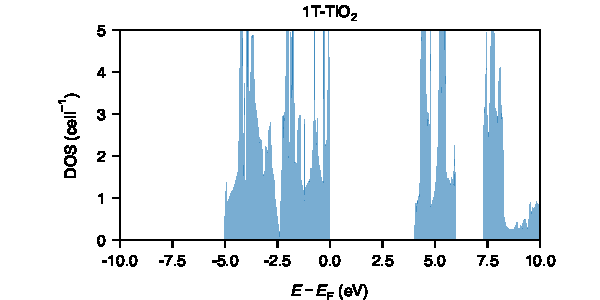
\includegraphics[width=.9\linewidth]{img/SI_figs/1T-TiO2-DOS.pdf}
\end{center}
\begin{center}
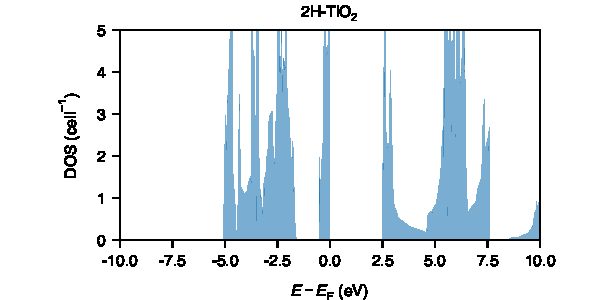
\includegraphics[width=.9\linewidth]{img/SI_figs/2H-TiO2-DOS.pdf}
\end{center}
\begin{center}
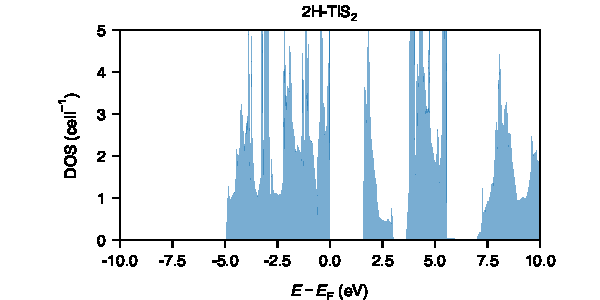
\includegraphics[width=.9\linewidth]{img/SI_figs/2H-TiS2-DOS.pdf}
\end{center}
\begin{center}
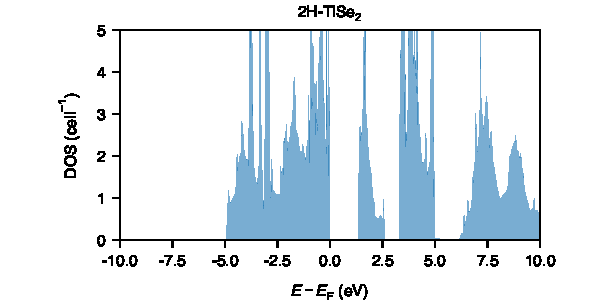
\includegraphics[width=.9\linewidth]{img/SI_figs/2H-TiSe2-DOS.pdf}
\end{center}
\begin{center}
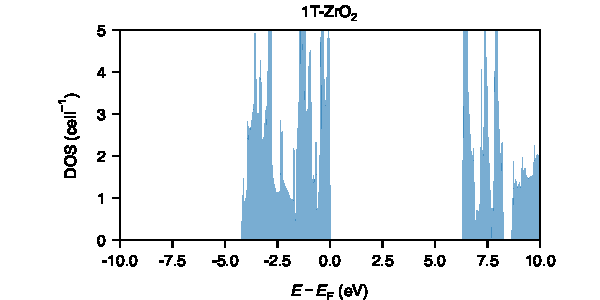
\includegraphics[width=.9\linewidth]{img/SI_figs/1T-ZrO2-DOS.pdf}
\end{center}
\begin{center}
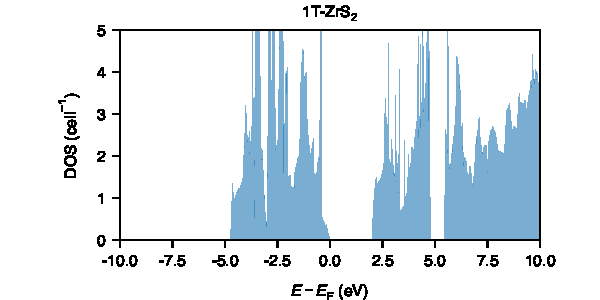
\includegraphics[width=.9\linewidth]{img/SI_figs/1T-ZrS2-DOS.pdf}
\end{center}
\begin{center}
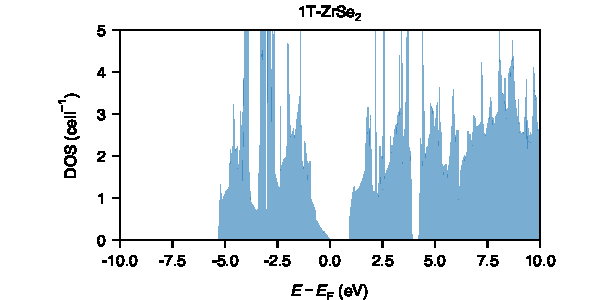
\includegraphics[width=.9\linewidth]{img/SI_figs/1T-ZrSe2-DOS.pdf}
\end{center}
\begin{center}
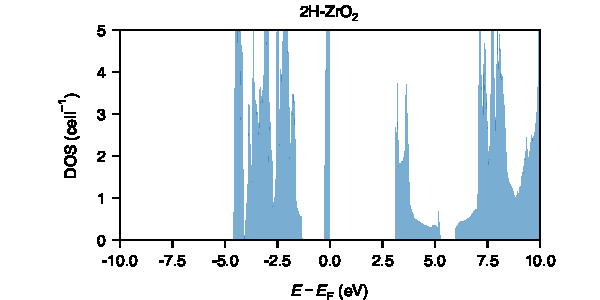
\includegraphics[width=.9\linewidth]{img/SI_figs/2H-ZrO2-DOS.pdf}
\end{center}
\begin{center}
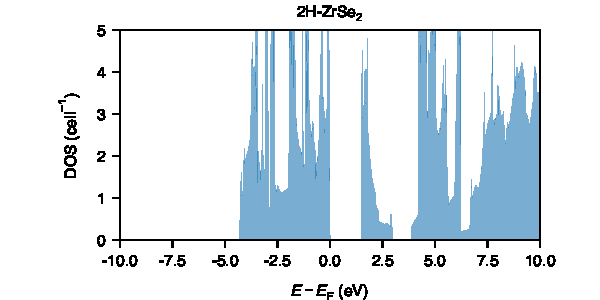
\includegraphics[width=.9\linewidth]{img/SI_figs/2H-ZrSe2-DOS.pdf}
\end{center}
\begin{center}
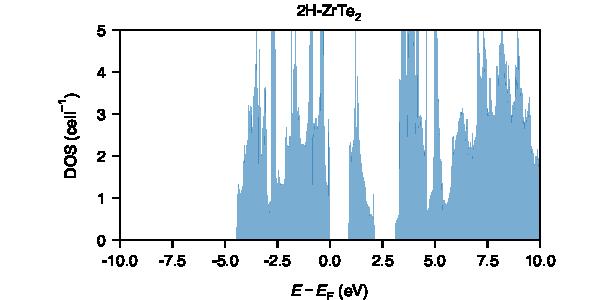
\includegraphics[width=.9\linewidth]{img/SI_figs/2H-ZrTe2-DOS.pdf}
\end{center}
\begin{center}
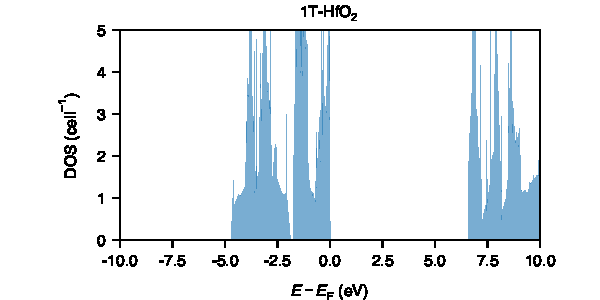
\includegraphics[width=.9\linewidth]{img/SI_figs/1T-HfO2-DOS.pdf}
\end{center}
\begin{center}
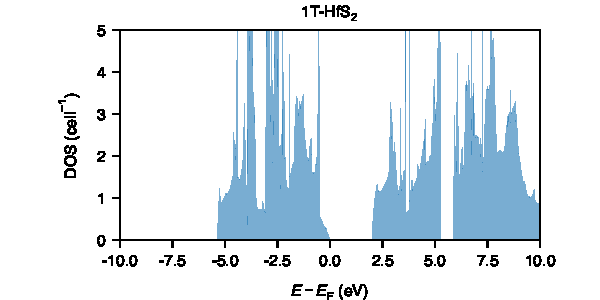
\includegraphics[width=.9\linewidth]{img/SI_figs/1T-HfS2-DOS.pdf}
\end{center}
\begin{center}
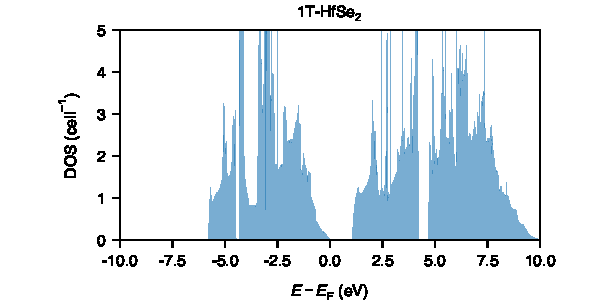
\includegraphics[width=.9\linewidth]{img/SI_figs/1T-HfSe2-DOS.pdf}
\end{center}
\begin{center}
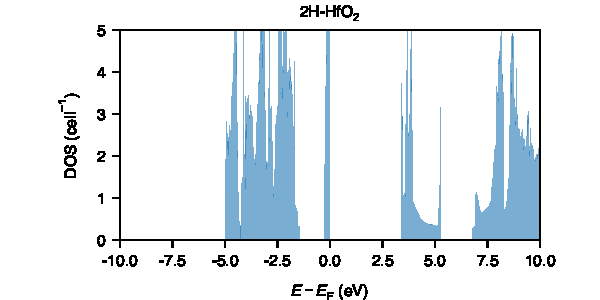
\includegraphics[width=.9\linewidth]{img/SI_figs/2H-HfO2-DOS.pdf}
\end{center}
\begin{center}
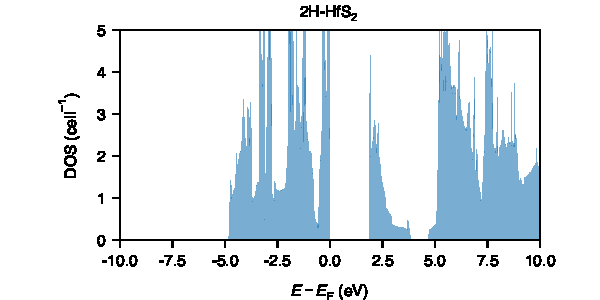
\includegraphics[width=.9\linewidth]{img/SI_figs/2H-HfS2-DOS.pdf}
\end{center}
\begin{center}
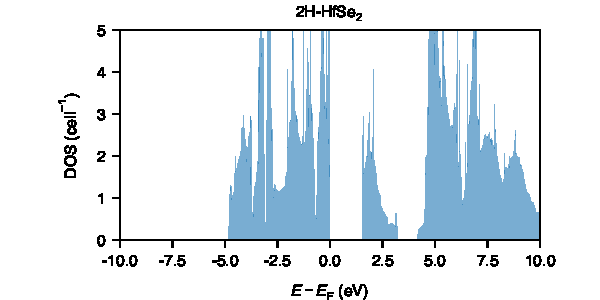
\includegraphics[width=.9\linewidth]{img/SI_figs/2H-HfSe2-DOS.pdf}
\end{center}
\begin{center}
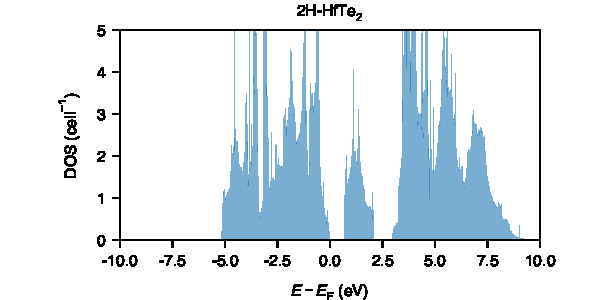
\includegraphics[width=.9\linewidth]{img/SI_figs/2H-HfTe2-DOS.pdf}
\end{center}
\begin{center}
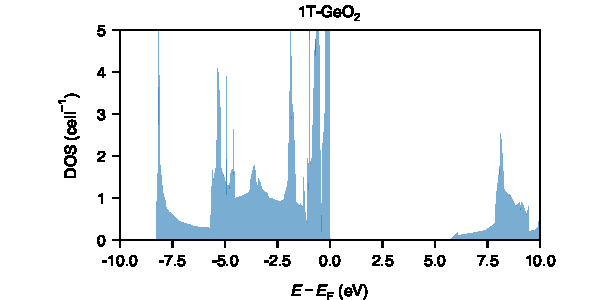
\includegraphics[width=.9\linewidth]{img/SI_figs/1T-GeO2-DOS.pdf}
\end{center}
\begin{center}
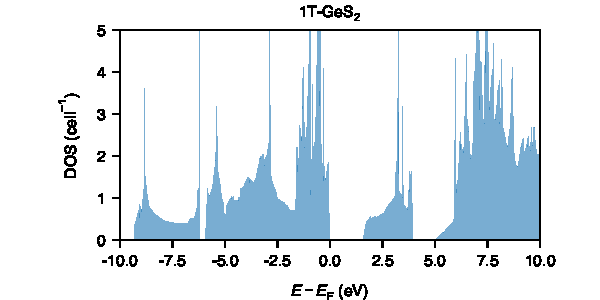
\includegraphics[width=.9\linewidth]{img/SI_figs/1T-GeS2-DOS.pdf}
\end{center}
\begin{center}
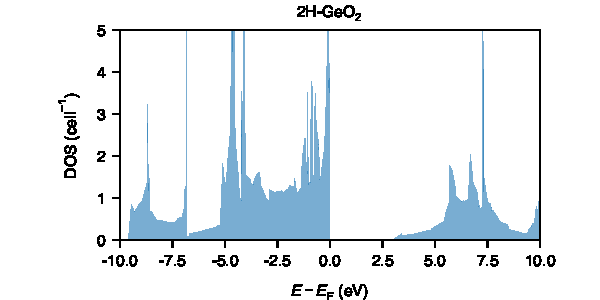
\includegraphics[width=.9\linewidth]{img/SI_figs/2H-GeO2-DOS.pdf}
\end{center}
\begin{center}
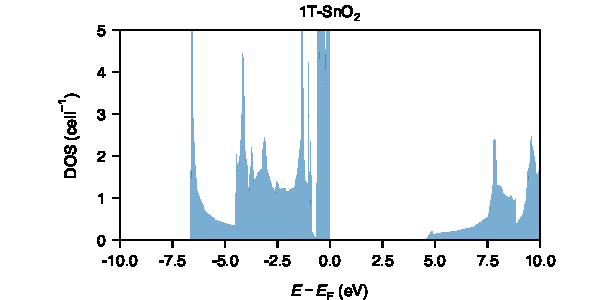
\includegraphics[width=.9\linewidth]{img/SI_figs/1T-SnO2-DOS.pdf}
\end{center}
\begin{center}
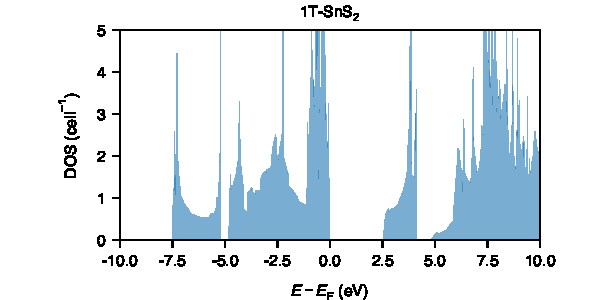
\includegraphics[width=.9\linewidth]{img/SI_figs/1T-SnS2-DOS.pdf}
\end{center}
\begin{center}
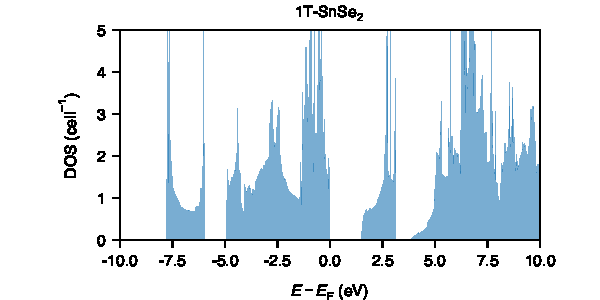
\includegraphics[width=.9\linewidth]{img/SI_figs/1T-SnSe2-DOS.pdf}
\end{center}
\begin{center}
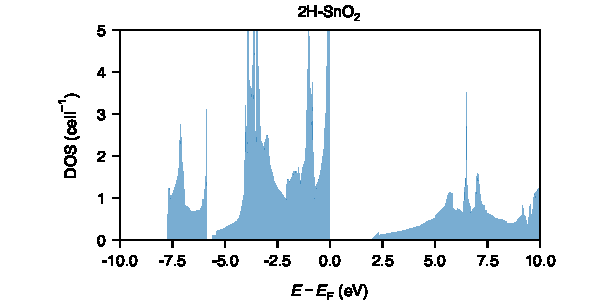
\includegraphics[width=.9\linewidth]{img/SI_figs/2H-SnO2-DOS.pdf}
\end{center}
\begin{center}
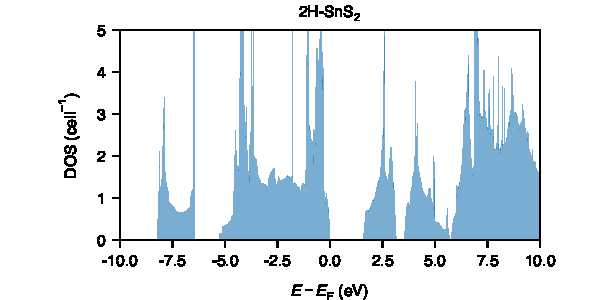
\includegraphics[width=.9\linewidth]{img/SI_figs/2H-SnS2-DOS.pdf}
\end{center}
\begin{center}
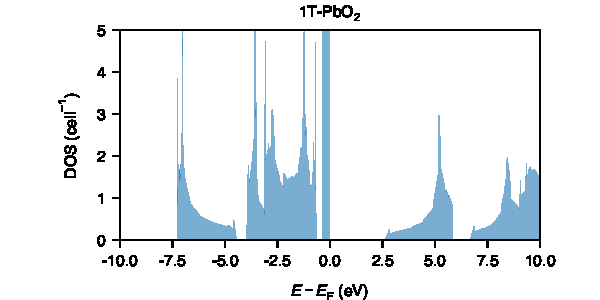
\includegraphics[width=.9\linewidth]{img/SI_figs/1T-PbO2-DOS.pdf}
\end{center}
\begin{center}
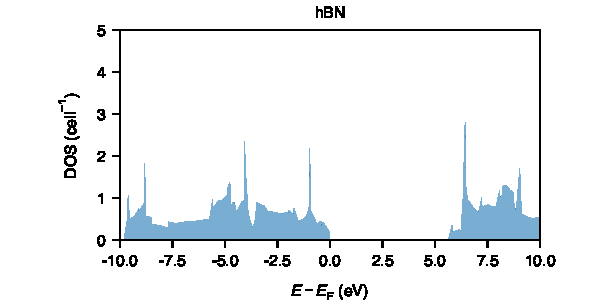
\includegraphics[width=.9\linewidth]{img/SI_figs/hBN-DOS.pdf}
\end{center}
\begin{center}
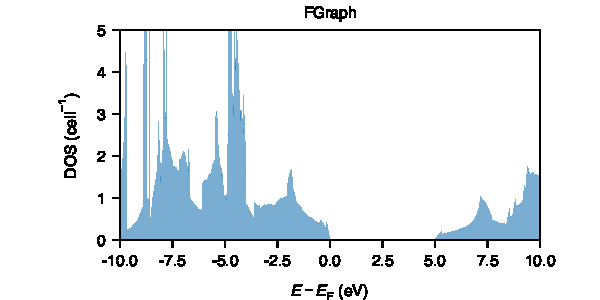
\includegraphics[width=.9\linewidth]{img/SI_figs/FGraph-DOS.pdf}
\end{center}
\begin{center}
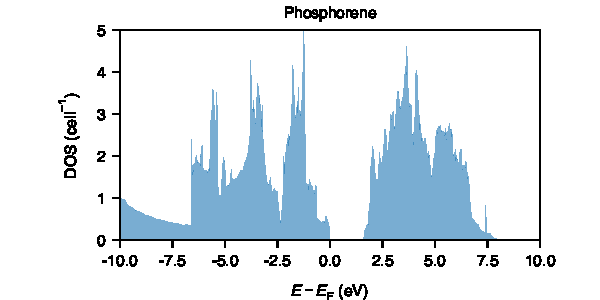
\includegraphics[width=.9\linewidth]{img/SI_figs/Phosphorene-DOS.pdf}
\end{center}
\begin{center}
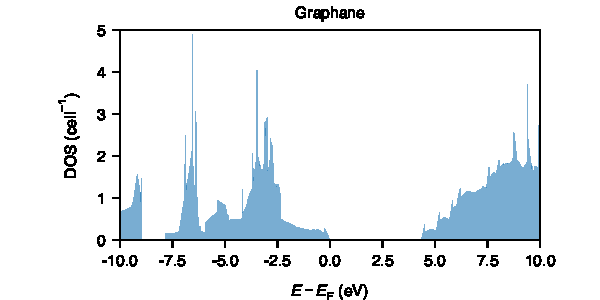
\includegraphics[width=.9\linewidth]{img/SI_figs/Graphane-DOS.pdf}
\end{center}
\begin{center}
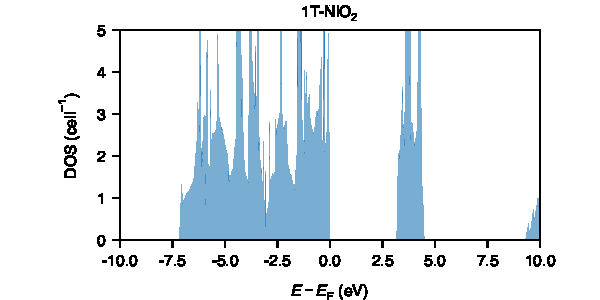
\includegraphics[width=.9\linewidth]{img/SI_figs/1T-NiO2-DOS.pdf}
\end{center}
\begin{center}
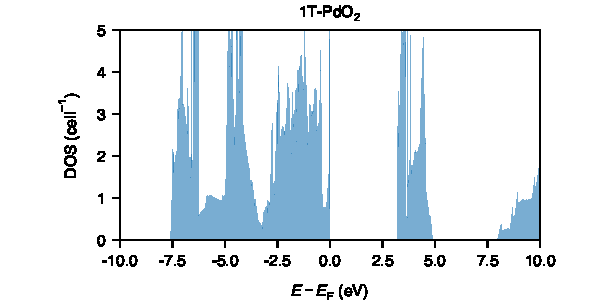
\includegraphics[width=.9\linewidth]{img/SI_figs/1T-PdO2-DOS.pdf}
\end{center}
\begin{center}
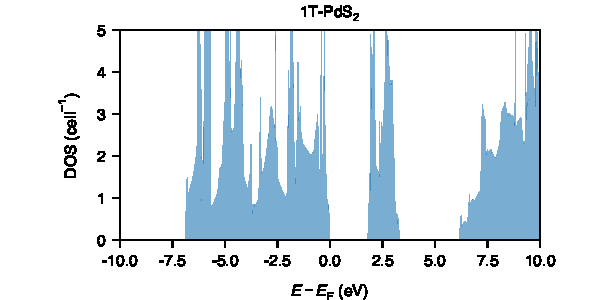
\includegraphics[width=.9\linewidth]{img/SI_figs/1T-PdS2-DOS.pdf}
\end{center}
\begin{center}
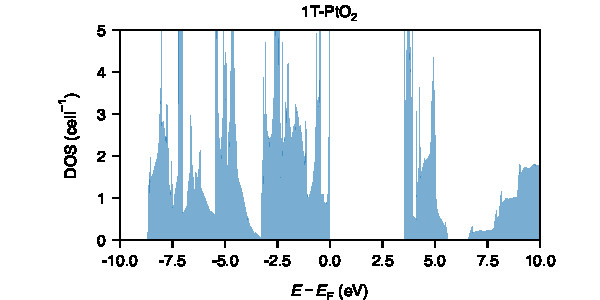
\includegraphics[width=.9\linewidth]{img/SI_figs/1T-PtO2-DOS.pdf}
\end{center}
\begin{center}
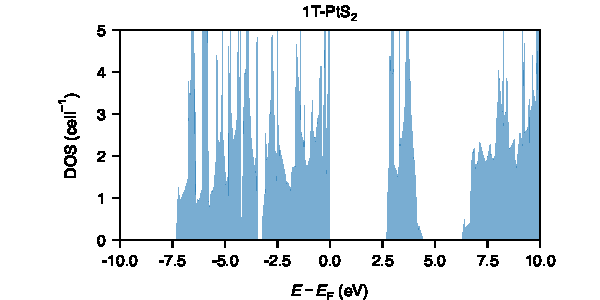
\includegraphics[width=.9\linewidth]{img/SI_figs/1T-PtS2-DOS.pdf}
\end{center}
\begin{center}
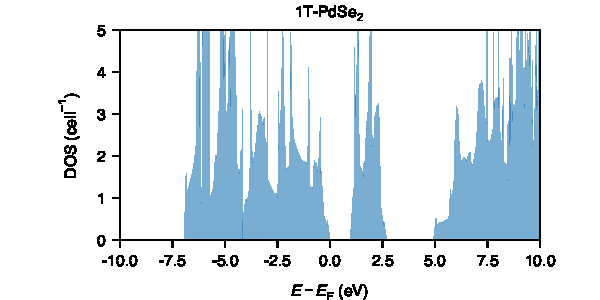
\includegraphics[width=.9\linewidth]{img/SI_figs/1T-PdSe2-DOS.pdf}
\end{center}
\begin{center}
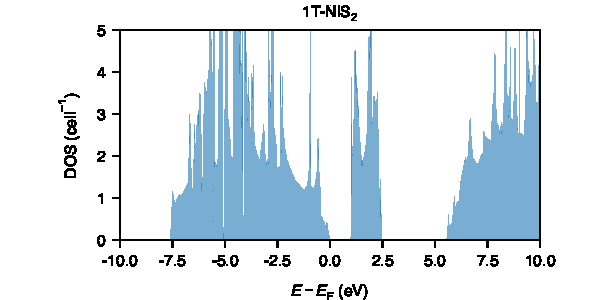
\includegraphics[width=.9\linewidth]{img/SI_figs/1T-NiS2-DOS.pdf}
\end{center}
\begin{center}
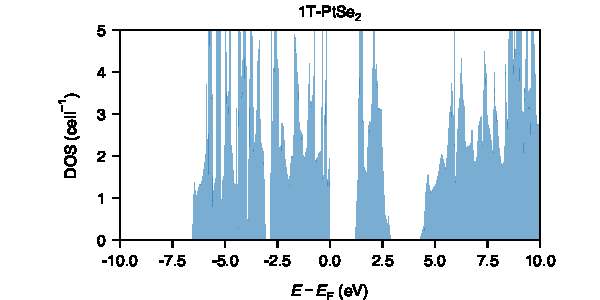
\includegraphics[width=.9\linewidth]{img/SI_figs/1T-PtSe2-DOS.pdf}
\end{center}
\begin{center}
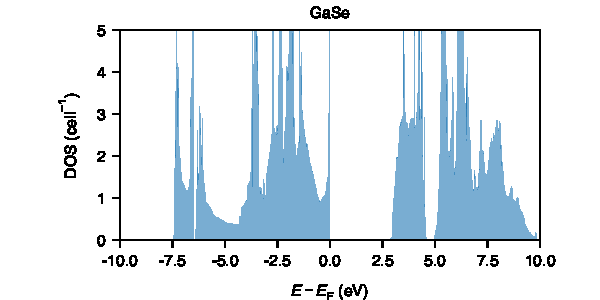
\includegraphics[width=.9\linewidth]{img/SI_figs/GaSe-DOS.pdf}
\end{center}
\begin{center}
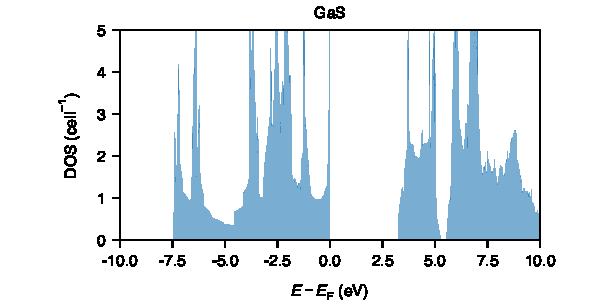
\includegraphics[width=.9\linewidth]{img/SI_figs/GaS-DOS.pdf}
\end{center}
\begin{center}
\includegraphics[width=.9\linewidth]{img/SI_figs/CdI2-DOS.pdf}
\end{center}
\begin{center}
\includegraphics[width=.9\linewidth]{img/SI_figs/2H-MoS2-DOS.pdf}
\end{center}
\begin{center}
\includegraphics[width=.9\linewidth]{img/SI_figs/2H-WS2-DOS.pdf}
\end{center}
\begin{center}
\includegraphics[width=.9\linewidth]{img/SI_figs/2H-WSe2-DOS.pdf}
\end{center}
\begin{center}
\includegraphics[width=.9\linewidth]{img/SI_figs/2H-WO2-DOS.pdf}
\end{center}
\begin{center}
\includegraphics[width=.9\linewidth]{img/SI_figs/2H-MoO2-DOS.pdf}
\end{center}
\begin{center}
\includegraphics[width=.9\linewidth]{img/SI_figs/2H-MoTe2-DOS.pdf}
\end{center}
\begin{center}
\includegraphics[width=.9\linewidth]{img/SI_figs/2H-WTe2-DOS.pdf}
\end{center}
\begin{center}
\includegraphics[width=.9\linewidth]{img/SI_figs/2H-CrS2-DOS.pdf}
\end{center}
\begin{center}
\includegraphics[width=.9\linewidth]{img/SI_figs/2H-CrSe2-DOS.pdf}
\end{center}
\begin{center}
\includegraphics[width=.9\linewidth]{img/SI_figs/2H-CrO2-DOS.pdf}
\end{center}


\pagebreak{}

\renewcommand\refname{Supplementary References}
\bibliography{ref_SI_v071618}

%\begin{thebibliography}{ref_SI_v012418}
%
%%\section*{Supplementary References}
%
%\end{thebibliography}

\end{document}

